\documentclass[UTF8]{ctexart}
\usepackage{SJTUSFFABookCover}  

%%--------------------版面参数--------------------%%
\newlength{\bleed}      \setlength{\bleed}{0mm}   % 出血
\newlength{\trimwidth}  \setlength{\trimwidth}{182mm} % 封面净宽
\newlength{\trimheight} \setlength{\trimheight}{257mm}% 封面净高
\newlength{\spinewidth} \setlength{\spinewidth}{7mm} % 书脊宽

%%--------------------纸张设置,已含出血--------------------%%
\geometry{
  paperwidth=\dimexpr\trimwidth+\spinewidth+\trimwidth+2\bleed\relax,
  paperheight=\dimexpr\trimheight+2\bleed\relax,
  margin=0pt
}

\pagestyle{empty}

\begin{document}
\begin{tikzpicture}[remember picture, overlay]

%%--------------------底图--------------------%%
  \node[anchor=south west, inner sep=0pt] at (current page.south west)
    {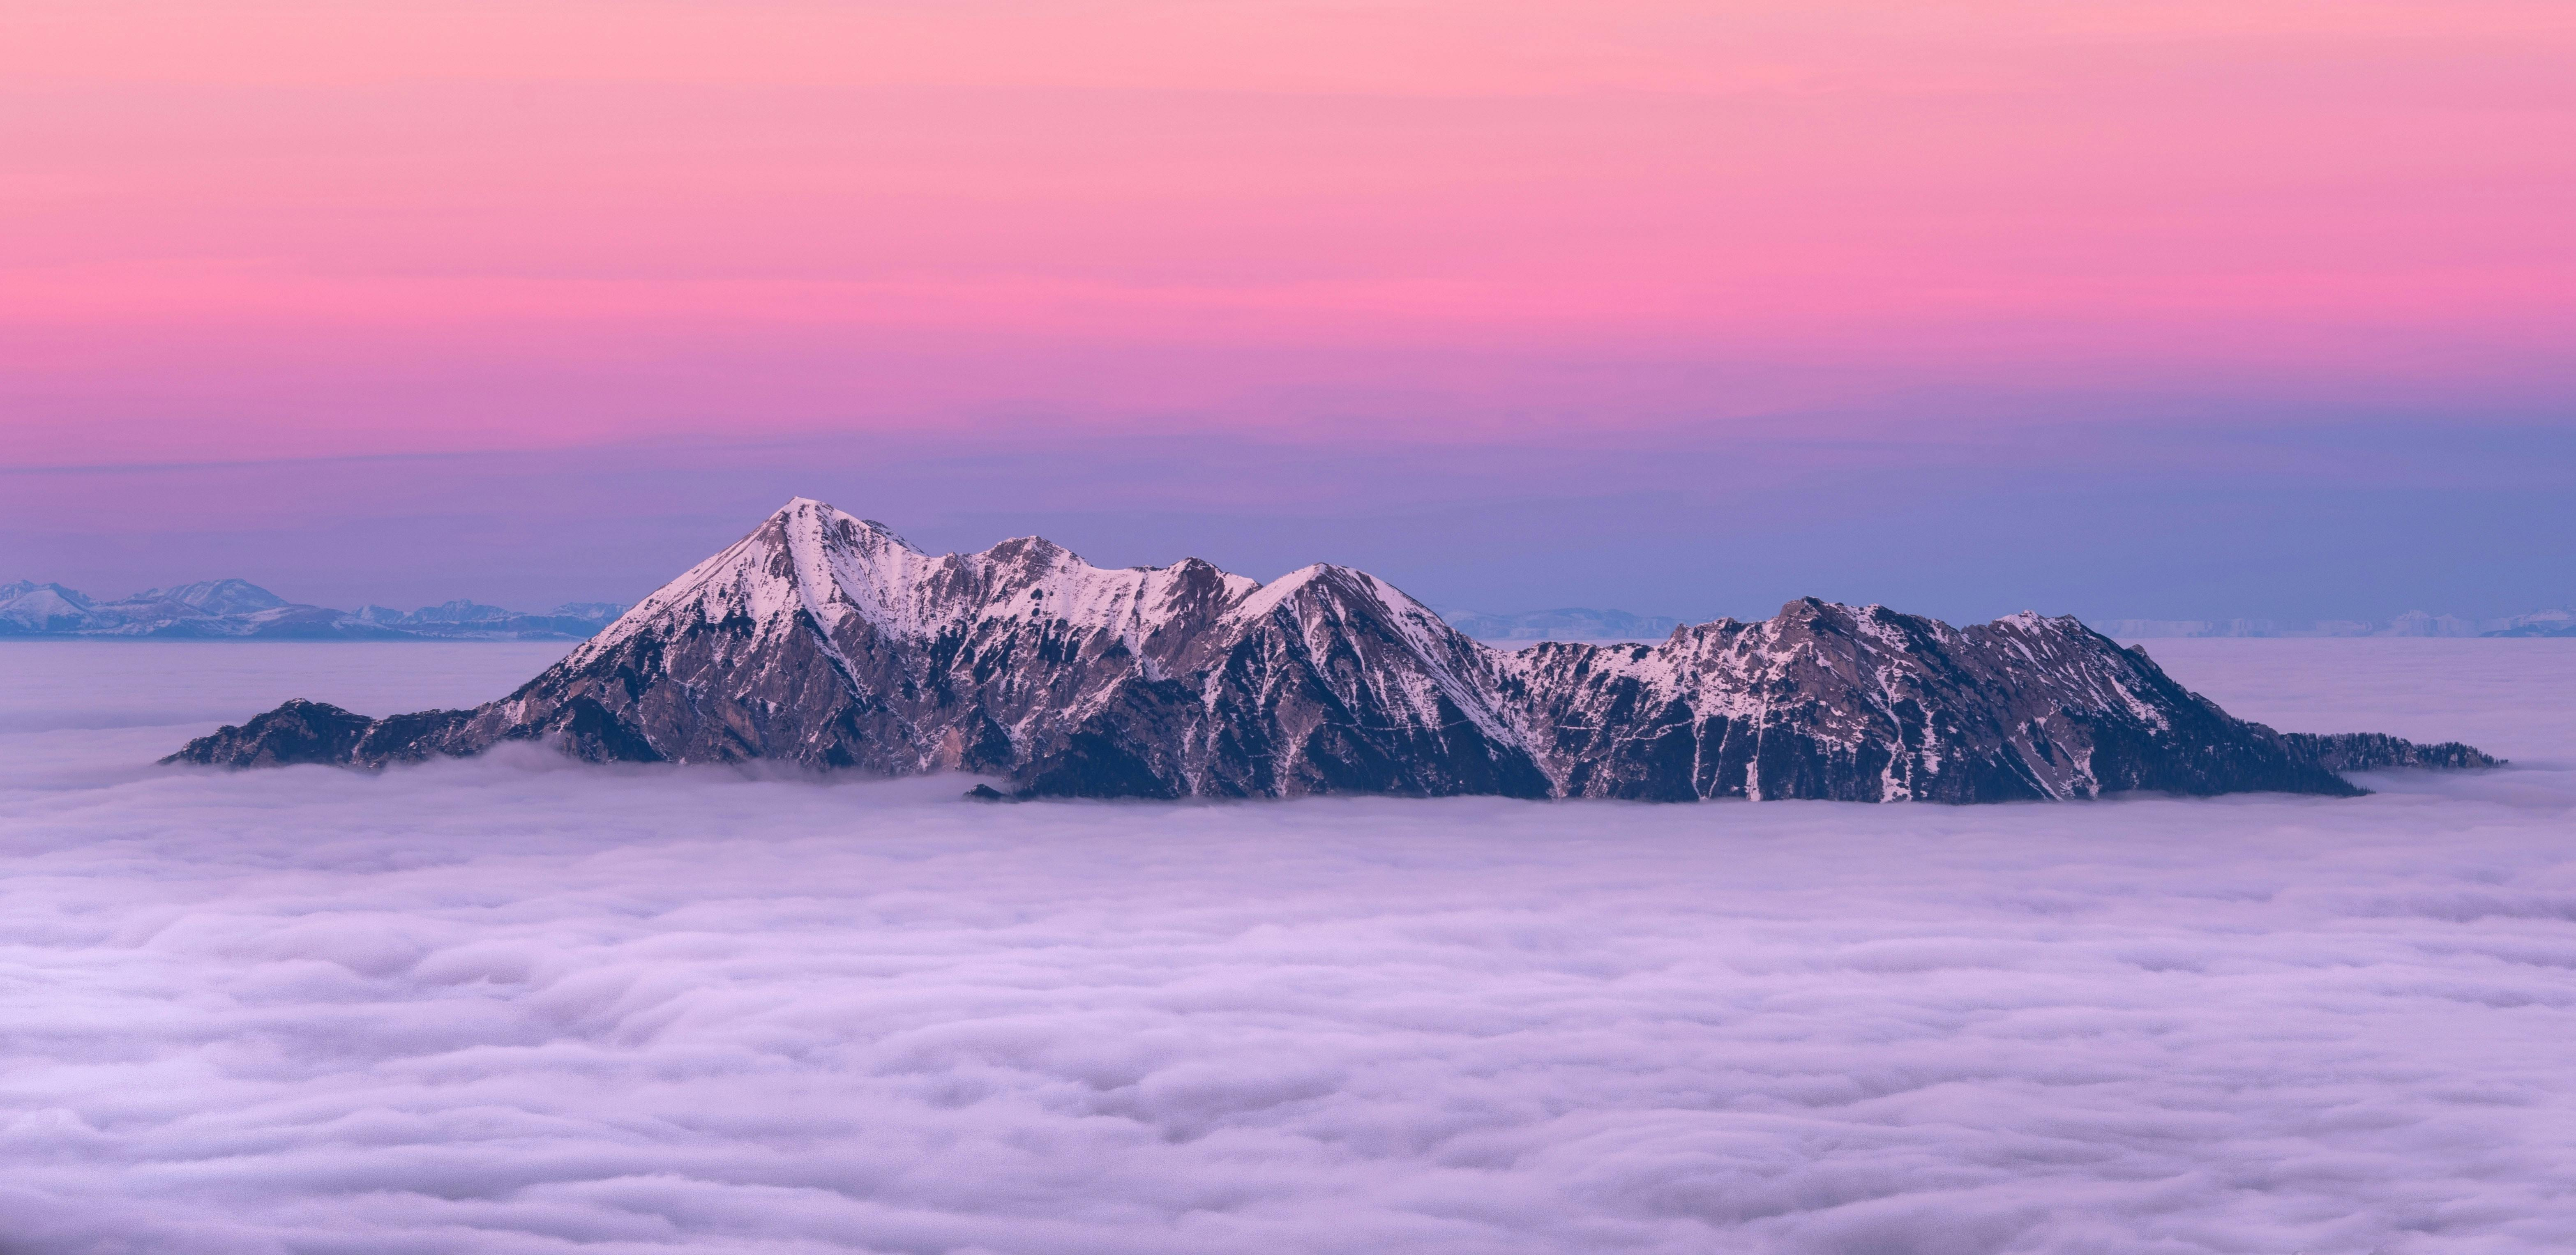
\includegraphics[width=\paperwidth,height=\paperheight]{cover.jpg}};

%%--------------------出血线--------------------%%
  \draw[gray,line width=1pt]
    ([shift={(\bleed,\bleed)}]current page.south west)
    rectangle
    ([shift={(-\bleed,-\bleed)}]current page.north east);
    
%%--------------------封底书脊封面分界线--------------------%%
%% 封底右边缘(书脊左)
    \draw[gray,line width=0.2pt]
    ([xshift=\bleed+\trimwidth]current page.south west)
    -- ([xshift=\bleed+\trimwidth]current page.north west);

%% 书脊右边缘(封面左)
  \draw[gray,line width=0.2pt]
    ([xshift=\bleed+\trimwidth+\spinewidth]current page.south west)
    -- ([xshift=\bleed+\trimwidth+\spinewidth]current page.north west);

%%--------------------封底(左侧)--------------------%%
  \node[anchor=south west, inner sep=0pt]
    at ([xshift=\bleed +4mm, yshift=\bleed ] current page.south west)  
    {
\includegraphics[width=84mm]{logo.png}};

%%--------------------书脊(中间)--------------------%%
  \node[
    rotate=-90,
    anchor=center,
    text=white,
    font=\fontsize{16}{24}\selectfont\timesnewroman
    ] at ([xshift=-\bleed-\trimwidth-\spinewidth/2,yshift=84mm] current page.east) % 仅横向平移
    {Live long and prosper};

  \node[
    rotate=0,
    anchor=center,
    text=white,
    align=left,
    font=\fontsize{16}{16}\selectfont\fzxztfw
    ] at ([xshift=-\bleed-\trimwidth-\spinewidth/2,yshift=-72mm] current page.east) % 仅横向平移
    {上\\海\\交\\通\\大\\学\\科\\幻\\奇\\幻\\协\\会};

%%--------------------封面(右侧)--------------------%%

%% 竖排英文
%% 阴影效果
  \node[
    rotate=-90,
    anchor=center, 
    text=black,
    font=\fontsize{300}{360}\selectfont\timesnewroman
    ] at ([xshift=-\bleed-44mm,yshift=-1mm] current page.east)
    {Y-H-J};

  \node[
    rotate=-90,
    anchor=center, 
    text=white,
    font=\fontsize{300}{360}\selectfont\timesnewroman
    ] at ([xshift=-\bleed-45mm] current page.east)
    {Y-H-J};

%% 竖排中文
  \node[
    rotate=0,
    anchor=center,
    align=left,
    text=black,
    font=\fontsize{48}{60}\selectfont\fzhfsjwh]
    at ([xshift=-\bleed-95.5mm,yshift=-0.5mm] current page.east)
    {生\\生\\不\\息\\繁\\荣\\昌\\盛};

  \node[
    rotate=0,
    anchor=center,
    align=left,
    text=white,
    font=\fontsize{48}{60}\selectfont\fzhfsjwh]
    at ([xshift=-\bleed-96mm] current page.east)
    {生\\生\\不\\息\\繁\\荣\\昌\\盛};


  
\end{tikzpicture}
\end{document}
